\documentclass[a4paper,10pt]{article}
\usepackage{src/preamble}

\begin{document}

\noindent
\begin{center}
	\textbf{{\Large MAGNETI SUPERCONDUTTORI}} \\
\end{center}

\noindent
\textbf{Autore: Alessandro Biagiotti} \textit{Università degli studi di Milano,
	Milano, Italia}
\\

\noindent
\textbf{INTRODUZIONE:}
\\
Come già introdotto nel documento dedicato alla parte teorica, in questo secondo documento mi
dedicherò a una trattazione più pratica delle tecnologie superconduttive che sono oggi più in
utilizzo nel campo della fisica delle alte energie, e non solo (basti pensare ad applicazioni
ingegneristiche per treni ad alta velocità \cite{maglev}).

I superconduttori sono materiali caratterizzati da un brusco annullamento della resistività ($R =
	0$ e non $R \approx 0$) una volta raggiunta una certa temperatura, nota come temperatura
critica.
\begin{figure}[h!]
	\centering

	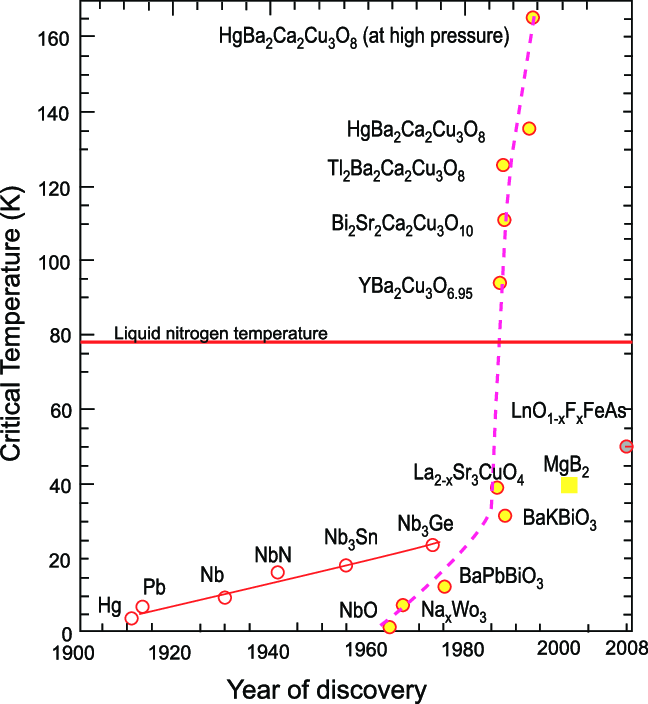
\includegraphics[scale=0.35]{fig/The-evolution-of-critical-temperatures-since-the-discovery-of-superconductivity.png}
	\caption{
		Temperatura critica di varie leghe che sono state scoperte nel corso degli anni
		\cite{critical-temp}
	}
\end{figure}
Il comportamento dei superconduttori puri è stato spiegato tramite la teoria BCS, risalente al
1957, l'azzeramento della resistività del materiale è dovuto alla formazione delle cosiddette
coppie di Cooper.

Una coppia di Cooper è una coppia di elettroni che viaggiano insieme ed è generata da
un'interazione tra un elettrone e il reticolo cristallino (che è carico positivamente).
Quest'interazione porta a uno sbilanciamento della carica locale che passa da negativa a positiva, è pertanto possibile che un altro elettrone venga attratto, dando vita a una coppia di
Cooper \cite{cooper-cambridge}. Una spiegazione più dettagliata del fenomeno mette in relazione
questo comportamento con uno scambio di fononi \cite{quantum-springer}.

In un normale conduttore la resistenza elettrica sarebbe generata dallo scattering degli elettroni
dovuto a collisioni con i nuclei positivi del reticolo cristallino. All'interno di un
superconduttore, però, la maggioranza degli elettroni sono coppie di Cooper. Queste coppie, sebbene
interagiscano con il reticolo cristallino, non ricevono abbastanza energia per spezzare il legame
che le tiene insieme e, di fatto, non si dividono negli elettroni che le formano. È per questo motivo che i superconduttori dimostrano di avere resistenza elettrica pari a zero \cite{bcs-cambridge}.

Sebbene la mancanza di resistenza possa far pensare che un superconduttore sia in grado di
supportare una quantità infinita di tensione e densità di corrente, si è scoperto, come si vedrà nel
seguito, che esistono altri limiti fisici che provocano la perdità della proprietà di
superconduttività.

All'interno di questo documento andrò ad esporre quali siano le tipologie di superconduttori
attualmente in esistenza e infine esplorerò alcune delle leghe più utilizzate e alcune tecnologie
più innovative nel campo della superconduzione a temperature elevate.

\bigskip
\phantomsection
\label{sec:type-one}
\noindent
\textbf{EFFETTO MEISSNER E TIPI DI SUPERCONDUTTORI:}
\\
Prima di poter introdurre la differenza tra superconduttori del primo e del secondo tipo bisogna
introdurre un'altra importante caratteristica dei superconduttori.

Questi, infatti, hanno un comportamento diamagnetico, il che significa che sono in grado di
espellere campi magnetici che normalmente li attraverserebbero. Questo comportamento, noto come
effetto Meissner, fu scoperto nel 1933 da Meissner e Ochsenfeld \cite{meissner}. Per quanto visto in
precedenza la resistenza all'interno di un superconduttore a temperatura inferiore a $T_c$ è $0$,
questo significa che in presenza di una certa densità di corrente $\ve{J}$ il campo elettrico
all'interno del conduttore può essere calcolato come:
\begin{equation}
	\ve{E} = R \times \ve{J} = \ve{0}
\end{equation}
Quindi se consideriamo la legge di Ampere-Maxwell
\begin{equation*}
	\curl{E} = - \pder{\ve{B}}{t} = 0
\end{equation*}
Quanto illustrato sopra porterebbe quindi a dire che il campo magnetico all'interno del
superconduttore è costante e quindi il flusso sarà a sua volta costante.

In realtà il lavoro di Meissner ha dimostrato che il comportamento del superconduttore è ben
diverso, infatti l'espulsione del campo magnetico deriva dalla presenza di "correnti di
schermatura"\footnote{screening currents} sulla superficie del superconduttore che generano un
campo magnetico opposto a quello imposto sul conduttore, cancellandone
l'effetto \cite{super-fundamentals}. Ulteriori studi da parte dei fratelli London dimostrarono che,
in realtà, vi è un certo livello di penetrazione del campo magnetico all'interno del conduttore, ma
l'intensità di quest'ultimo scala esponenzialmente con la distanza di penetrazione all'interno del
materiale \cite{ssp}.

\bigskip
\noindent
I materiali superconduttori, sulla base di come si comportano in presenza di un campo magnetico
esterno, sono di tipo I o tipo II.

Tutti i materiali superconduttori di tipo I presentano una linea di demarcazione forte tra lo stato
di repulsione del campo magnetico (\emph{meissner state}) e lo stato di "permeazione" del campo
magnetico (\emph{normal state}). Questa caratteristica è resa evidente da Figura \ref{fig:phase-diagram}.
\begin{figure}[h!]
	\centering

	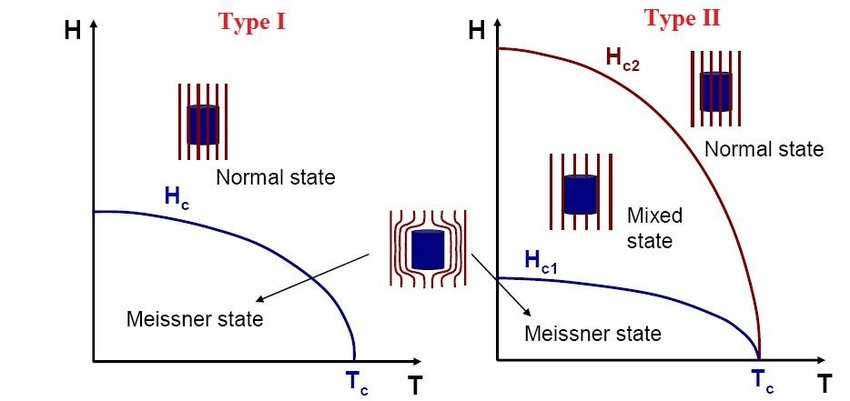
\includegraphics[scale=0.35]{fig/phase-diagram.jpg}
	\caption{
		Diagrammi di fase per superconduttori di tipo I e tipo
		II\cite{super-types}
	}\label{fig:phase-diagram}
\end{figure}

I conduttori di secondo tipo furono scoperti sperimentalmente in da una ricerca del 1937 \cite{type-2} e la teoria ad essi associata fu ulteriormente ampliata da interpretazioni nel regno della meccanica quantistica nei decenni a seguire. La necessità di nuove teorie e spiegazioni era dettata dal comportamento ibrido dei superconduttori del secondo tipo (mostrato in Figura \ref{fig:phase-diagram}), questi infatti:
\begin{itemize}
	\item Hanno uno stato superconduttivo.
	\item Hanno un \emph{meissner state}.
	\item Hanno uno stato ibrido in cui il campo permea parzialmente la superficie del magnete.
\end{itemize}
Delle nuove teorie erano necessarie per essere in grado di spiegare questo stato ibrido tra superconduttività e normal-conduttività.

Quando un superconduttore del secondo tipo entra nello stato ibrido viene concessa la penetrazione del campo magnetico all'interno della superficie in certi punti del superconduttore, in virtù della struttura che si viene a formare sono noti come vortici, mentre in altri la resistenza rimane a $0$. Il comportamento in prossimità dei vortici diviene normal-conduttivo e (come succedeva per i superconduttori del primo tipo) si generano delle \emph{screening currents} che vorticano\footnote{Ecco da dove viene il nome vortice usato in precedenza} intorno al punto di penetrazione e si oppongono alla presenza del campo all'interno del superconduttore.

Siccome, per definizione, la corrente elettrica prende il percorso di minor resistenza il conduttore risulta comunque avere resistenza $0$ (anche con una parziale penetrazione del campo magnetico al suo interno), affinchè il superconduttore possa rimanere in una situazione di perdita $0$ è necessario fare in modo che i vortici rimangano fissati a impurità del reticolo cristallino.

\bigskip
\phantomsection
\label{sec:metallurgy}
\noindent
\textbf{CENNI DI METALLURGIA:}

\clearpage

\printbibliography

\end{document}